\documentclass[12pt]{article}
\usepackage{graphicx}
\usepackage{graphics}
\usepackage{refstyle}
\usepackage{amsmath}
\usepackage{caption}
\usepackage{float}
\usepackage{booktabs}
\usepackage{array}
\usepackage{amssymb}
\usepackage{booktabs}
\renewcommand{\vec}{\boldsymbol}
\providecommand{\brak}[1]{\ensuremath{\left(#1\right)}}
\graphicspath{{/storage/self/primary/Download/latexnew/fig}}                                            
\graphicspath{{/storage/self/primary/Download/latexnew/table}}
\begin{document}
\title{\textbf{VECTOR}}
\date{}
\maketitle
\textbf{Question:} $\vec{P}$ and $\vec{Q}$ are any two points lying on the sides $DC$ and $AD$ respectively of a parallelogram $ABCD$.Show that, $ar\brak{\triangle APB}=ar\brak{\triangle BQC}$.


\textbf{Figure:}
\begin{figure}[H]
    \centering
   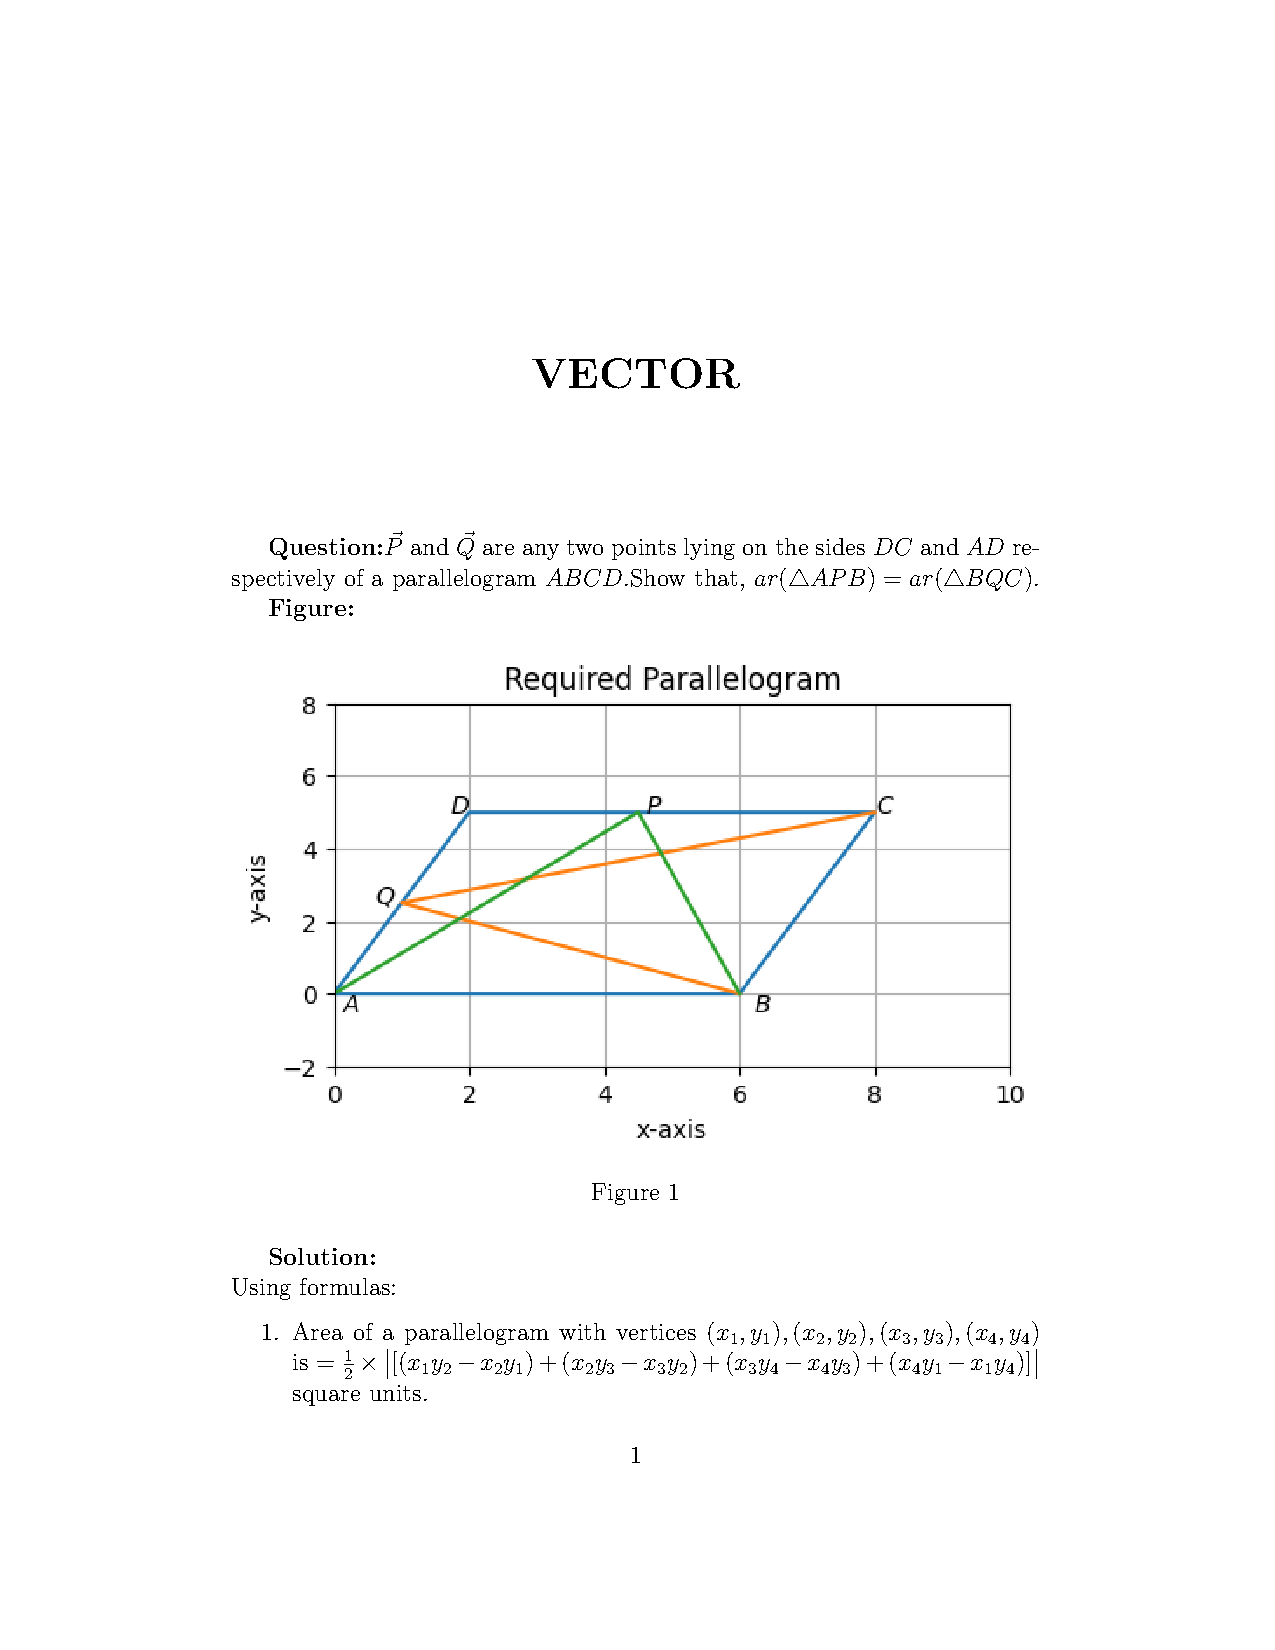
\includegraphics[width=\columnwidth]{fig/1.png}
    \caption{}
    \label{fig:fig:1}
\end{figure}


\textbf{Solution:}\\
From \figref{fig:1} ,
considering $\triangle BQC$ and parallelogram $ ABCD$, having \underline{same base $BC$} and, \underline{$AD$ is parallel to $BC$}.\\
\begin{align}
\implies \triangle BQC = \frac{1}{2}\times ar ABCD.
  \label{eq:eq:1}
\end{align}
Considering $\triangle APB$ and parallelogram $ABCD$ , having \underline{same base $AB$} and,\underline{$DC$ is parallel to $AB$}.

\begin{align}
\implies \triangle APB = \frac{1}{2}\times ar ABCD.
\label{eq:eq:2}
\end{align}

By comparing \eqref{eq:1} and \eqref{eq:2} we obtain that,

\begin{align}
    ar\brak{\triangle APB} =  ar\brak{\triangle BQC}.
\end{align}
\begin{center}
 Hence proved.

\end{center}

\textbf{Proof by the help of diagram :}\brak{\figref{fig:1},\tabref{tab:1},\tabref{tab:2}}\\
Let the points $\vec{Q}$ and $\Vec{P}$ divide $AD$ and $CD$ by $k_1:1$ and $k_2:1$ ratio respectively.
\begin{table}[H]
   \centering
      \begin{tabular}{|c|c|c|}
    \hline
    \textbf{Input Parameters} &\textbf{Description} &\textbf{Value} \\
    \hline
     $\vec{O}$& Center(at origin)&$\vec{0}$\\
     \hline
 $r$ & Radius &1\\
 \hline
 $\theta$&-&$100\degree$\\
 \hline
 $\alpha$&-&$165.4\degree$\\
 \hline
 $\beta$&-&$5\degree$\\
 \hline
  \end{tabular}

   \caption{Table of input parameters}
   \label{tab:tab:1}
\end{table}




\begin{table}[H]
    \centering                                      
    \begin{tabular}{|c|c|c|}
    \hline
        \textbf{Output Parameters} &\textbf{Description} &\textbf{Value} \\
\hline
          $\vec{Q}$ & Point &$\myvec{\cos{\theta_1}\\\sin{\theta_1}}$\\
          \hline
          $\vec{P}$ & Point &$\myvec{\cos{\theta_2}\\\sin{\theta_2}}$ \\
         \hline
          $\vec{R}$ & Point &$\myvec{\cos{\theta_3}\\sin{\theta_3}}$ \\
         \hline
    \end{tabular}

                          
    \caption{Table of output parameters}
	\label{tab:tab:2}
 \end{table}


For the $\triangle BQC$, the vertices of the triangle are
$\Vec{B}=\begin{pmatrix}
       6\\0
   \end{pmatrix},
   \Vec{Q}=\begin{pmatrix}
       \frac{2k_1}{k_1+1}\\\frac{5k_1}{k_1+1}
   \end{pmatrix},
   \Vec{C}=\begin{pmatrix}
       8\\5
   \end{pmatrix}$\\
$\implies\triangle BQC =
\begin{tabular}{|c c c|}
       1 &1&1\\
       6&$\frac{2k_1}{k_1+1}$&8 \\
       0&$\frac{5k_1}{k_1+1}$&5
   \end{tabular}\\
= \frac{1}{2} \times \big|1\brak{\frac{2k_1}{k_1+1}.5-\frac{5k_1}{k_1+1}.8}-6\brak{5.1-\frac{5k_1}{k_1+1}.1}+0\big|\\
 = \frac{1}{2} \times\big |\frac{-40k_1+10k_1-30}{k_1+1}\big|\\
 =\frac{1}{2} \times30\\
 =15 $square  units.

For the $\triangle APB$, the vertices of the triangle are

   $\Vec{A}=\begin{pmatrix}
       0\\0
   \end{pmatrix},
   \Vec{P}=\begin{pmatrix}
       \frac{8k_2+2}{k_2+1}\\5
   \end{pmatrix},
   \Vec{B}=\begin{pmatrix}
       6\\0
   \end{pmatrix}$\\
   $\implies \triangle APB =
   \begin{tabular}{|c c c|}
       1 &1&1\\
       0&$\frac{8k_2+2}{k_2+1}$&6 \\
       0&5&0
   \end{tabular}\\
 = \frac{1}{2} \times \big |1\brak{\frac{8k_2+2}{k_2+1}.0-6.5}+0+0\big|\\
 = \frac{1}{2} \times\big |-30\big|\\
 =\frac{1}{2} \times30\\
 =15 $ square units.


 
  For parallelogram $ABCD$,the vertices are

   $\Vec{A}=\begin{pmatrix}
       0\\0
   \end{pmatrix},
 \Vec{B}=\begin{pmatrix}
       6\\0
   \end{pmatrix},
   \Vec{C}=\begin{pmatrix}
       8\\5
   \end{pmatrix},
   \Vec{D}=\begin{pmatrix}
       2\\5
   \end{pmatrix}$
   
$\implies ar ABCD = ab\sin\theta$\\
 =$6\sqrt{29}\sin\brak{\sin^{-1}{\frac{5}{\sqrt{29}}}}$\\
=$6\sqrt{29}\frac{5}{\sqrt{29}}$\\
=30 square units.


 Therefore,$ar ABCD = 2\times ar\triangle APB = 2\times ar \triangle BQC$\brak{proved}.\\
 


\end{document}

